\chapter{Development}
\section{Initial testing}
\subsection{Storing questions - Regex}
One of the features that the program requires is an ability to generate random questions. An initial idea was to just store the questions in a text file.
\begin{figure}[H]
	\centering
	\texttt{A ball is projected with speed 20 ms$^{-1}$. At the starting point the ball is 12m of the ground. The highest point of the ball is 20m. Find theta.}
	\caption{Initial question store}
\end{figure} 
The problem with this method is that it is hard to randomise the question. This is because the parts to be randomised in the string are not easily identifiable. 
\begin{figure}[H]
	\centering
	\texttt{A ball is projected with speed [speed]. At the starting point the ball is [height] of the ground. The highest point of the ball is [highpoint]. Find theta.} 
	\caption{Question store with identifiable variables}
\end{figure}
Now the variables can be differentiated from other text, this allows a regular expression to be constructed. The regular expression  will return text enclosed by brackets.
\begin{figure}[H]
	\texttt{import re\\
		question = "A ball is projected with speed [speed]."\\
		variables = re.findall(r'\textbackslash [\textbackslash w+\textbackslash ]', question)\\
		print(variable)\\
		>>> ['[speed]']}
	\caption{Extracting variables from a string using Python regex}
\end{figure} 
This shows how the variables could be extracted using python code. A random number could then be inserted using \texttt{random.randint(range)} function. 

There are downsides to using regular expressions. While it is easy to generalise areas of the string that you would like to capture, the expression can get very complex and hard to maintain. I don't think that I have sufficient experience in using regular expressions to be able to confidently use them in this project, so this method was discarded.
\subsection{Storing questions - String formatting}
Python has built in methods to format strings. This is shown in Figure 2.3 found in Section 2.5.4. This functionality is quite basic, and does not allow you to extract the name of the identifiable variable stored in the string (Figure 3.2). This means that it is hard to extract the name of the variable.

Fortunately there is a way to extend the functionality of the inbuilt Python string formatter, so that it can be customised to your needs. More details about that can be found in PEP 3101\autocite{pep3101}. This shows that you can create a class, that takes a string as an input, and formats the text however you would like it to. 

\begin{figure}[H]
\begin{lstlisting}[language=Python,]
	class object:
	  def __format__(self, format_spec):
	    return format(str(self), format_spec)
\end{lstlisting}
\caption{Example of extended string formatting\autocite{pep3101}}
\end{figure}

This shows how much you can custom the string formatter. An example string for use in this is shown in Figure 2.4.

This method was chosen for use in the project.

\subsection{Graph generation}
There are many Python libraries that allow you to plot graphs and draw diagrams. The most popular library is Matplotlib, which was initially created in 2002 by John Hunter. It allows data to be plotted in a highly customisable way, and interacts very well with Python arrays, which is useful when the data being plotted is generated at runtime.

\begin{figure}[H]
	\centering
	\begin{lstlisting}[language=Python]
	import matplotlib.pyplot as plt
	plt.plot([1,2,3,4])
	plt.ylabel('some numbers')
	plt.show()
	\end{lstlisting}
	
	\caption{Code to create Figure 3.6 \autocite{mpl}}
\end{figure}
This is code used to generate the simple graph seen below.
\begin{figure}[H]
	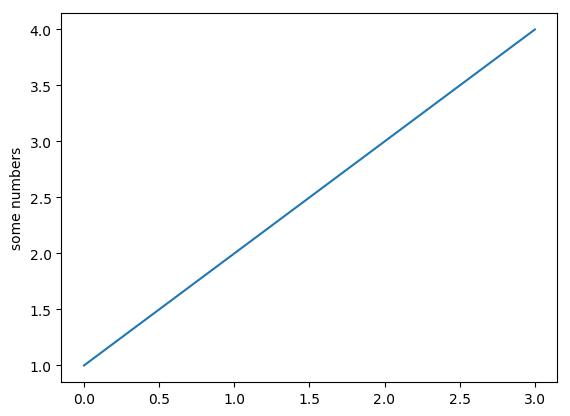
\includegraphics[width=\textwidth,height=\textheight,keepaspectratio]{exmpl.png}
	\caption{Graph generated by code in Figure 3.5}
\end{figure}
The code in Figure 3.5 shows how easy it is to draw a clean looking graph, which would be suitable for use in the program.

Other Python plotting libraries were not looked at, as Matplotlib is perfect for the needs of the project. It is also part of the Anaconda platform\autocite{conda} which is a Python installation containing many scientific Python libraries.  This library was chosen for use in the project.

\subsection{GUI}
There are hundreds of libraries to display GUI's in Python, but there are three that are most commonly used which are:
\begin{itemize}
	\item Tkinter
	\item PyQT
	\item WxPython
\end{itemize}
These are all Python wrappers for C/C++ code, which can make development hard because in some cases error codes may not be returned to the Python console, so you don't know what you have done wrong.

WxPython was immediately discounted, as it does not have stable support for Python version 3.x .

Next tkinter was considered. tkinter is a Python wrapper of Tcl/tk. It is class based, so to create a GUI you must create a class that extends the base frame class, and to customise this frame, you must override methods from the parent class. While the code is not that complex itself, the positioning of elements can get very complex, as it must be done entirely in code, as there is no WYSIWYG\footnote{What you see is what you get.} editor. As this project has a time constraint, tkinter was discarded.

Lastly PyQt was looked at. PyQt is a Python wrapper for Qt, which is a highly popular GUI framework, which is even used for the main touchscreen in the Tesla Model S. Qt comes with an excellent WYSIWYG editor, allowing you to easily create a GUI without having to worry about the code behind it. The code generated however is in C, which would be hard to integrate with the other Python code.

Luckily, there is a program called PyUIC5, which converts C code used to display a Qt GUI, into Python code that performs exactly the same function. This is the perfect tool for this project, as it allows the GUI to be created easily, and functionality to be easily added to the buttons, by extending some classes in the Python code.

Here is how the GUI design workflow will work with PyQt:
\begin{enumerate}
	\item Design GUI in QtCreator
	\item Convert generated C code into Python
	\item Add functionality to buttons in Python code
\end{enumerate}

PyQt was chosen as the GUI tool.

\subsection{Summary}
\begin{itemize}
	\item Extending the Python string formatter for storing questions
	\item Matplotlib for drawing the graphs
	\item PyQt for displaying the GUI
\end{itemize}
\section{Storing questions}
I decided to code each element of the program separately, and then once they are working on their own, to integrate them into the final project. I started writing the question store code first, as it just used vanilla Python, so I didn't have to worry about trying to install libraries. 

The code for overriding the Python string formatter was implemented first.
\begin{lstlisting}[language=Python, caption=Formatter override]
#RandomizedFormatter class. Child of Randomized class. Overrides String formatter to allow
#question formatting.
class RandomizedFormatter(object):
	def __init__(self, name, args):
		self.name = name
		self.args = args

	#This function overrides the Python string formatter.
	def __format__(self, fmt):
		op, rest = fmt.split(':', 1)
		
		if op == 'type':
			self.args[self.name] = rest
			return ""
		elif op == 'random':
			low, high = rest.split(':')
			value = random.randint(int(low), int(high))
			self.args[self.name] = value
			return str(value)
\end{lstlisting}
This piece of code overrides the Python string formatter. It then formats the question with this algorithm:
\begin{itemize}
	\item Find text enclosed by curly braces and place into a list.
	\item Split the text at the colons.
	\item Determine what the operator is.
	\item Format the text according to the operator.
	\item Store the randomized variable.
\end{itemize}
The operators available are \texttt{type}, and \texttt{random}. If the operator is type, then in the questionstore file the variable will look like this \texttt{\{equation:type:equationtype\}}. This allows the program to know which equation to use with the data it is given.

For the \texttt{random} operator, the variable will look like this \texttt{a:random:5:30} where \texttt{a} is the name of the variable that the random value will be stored in, \texttt{random} is the operator, and \texttt{5:30} is the range for the random number generation. 

Now that the code for formatting the string is complete, it was decided to create a parent class which would have other methods. This class would have to be able to return the answer to the question, the values of the randomly generated variables, and also the formatted string. This is the first version of the code for this.
\begin{lstlisting}[language=Python, caption=questionStore Parent Class v1]
class Randomized(object):
	def __init__(self):
		self.args = {}
		self.question = None
	
	#Returns the value of the randomized variable in the string.
	def __getitem__(self, name):
		return RandomizedFormatter(name, self.args)
	
	#Formats the string, using the overridden method found in the RandomizedFormatter class.
	def format(self, s):
		return string.Formatter().vformat(s, args=(), kwargs=self)
	
	#Returns the question class depending on the equation type.
	def get_class(self):
		if self.args['equation'] == "findtheta":
			self.question = questionplotclass.ProjectileQuestion(self.args['b'], self.args['a'], random.randint(40, 60))
			answer = self.question.answer_theta()
			return answer
		if self.args['equation'] == "findmaxheight":
			self.question = questionplotclass.ProjectileQuestion(self.args['c'], self.args['a'], self.args['b'])
			answer = self.question.answer_max_height()
			return answer
		if self.args['equation'] == 'findxdistance':
			self.question = questionplotclass.ProjectileQuestion(self.args['c'], self.args['a'], self.args['b'])
			answer = self.question.answer_xdistance
			return answer
\end{lstlisting}
This code couldn't be properly tested, as the \texttt{questionPlotClass} hadn't been written yet, so random numbers were given as answers for testing. While this code returns the answer, there is a problem because when the class is initialised, a random number is used, and this is not stored. This means that if another method wants to be called on the class, it will most likely have a different result, as the random number generated will be different.

This problem was solved by instead of just returning the answer, the instance of the class was returned. This meant that any method could be called on this instance of the class, without having to store the random number. 

A function was also added to retrieve a random line from a text file of questions. This is the \texttt{load} 
The second version of the \texttt{get\_class} function:
\begin{lstlisting}[language=Python, caption=Second iteration of the get\_class function]
#Returns the question class depending on the equation type.
def get_class(self):
	if self.args['equation'] == "findtheta":
		self.question = questionplotclass.ProjectileQuestion(self.args['b'], self.args['a'], random.randint(40, 60))
		self.question.find_theta()
		return self.question
	if self.args['equation'] == "findmaxheight":
		self.question = questionplotclass.ProjectileQuestion(self.args['c'], self.args['a'], self.args['b'])
		self.question.find_max_height()
		return self.question
	if self.args['equation'] == 'findxdistance':
		self.question = questionplotclass.ProjectileQuestion(self.args['c'], self.args['a'], self.args['b'])
		self.question.find_xdistance()
		return self.question
\end{lstlisting}
You can see that this code now returns the instance of the class instead of the answer.

Now that both the parent and child class were complete, they were put together to make the final Python file for the question formatting.
\lstinputlisting[language=Python, caption=Final questionStore code]{../questionStore.py}
Here is a list of features that this piece of code performs:
\begin{itemize}
	\item Formats a question string by replacing variables with random numbers and storing value.
	\item Allows the instance of the class used to display the question to be returned so other methods can be called on it.
	\item Loads a random question string from a text file.
\end{itemize} 
\section{Graph Generation}
After the code for string formatting was completed, next the code for the graph generation was made. This code is linked to the question generation, as it requires the random variables, and the equations used to generate the graph can also be used to create an answer.
\subsection{Equations}
To generate the graphs, a series of coordinates that the particle will pass through need to be calculated. matplotlib will then draw a smooth curve between these points. To keep things simple, and similar to the A2 Maths and Physics syllabus air resistance is ignored. So the horizontal speed won't change, and can be written as \[v_x = u\cos\theta\] where $u$ is the initial speed, and $\theta$ is the angle the particle is launched to the horizontal. The position can then be calculated by using distance = speed x time, so the equation for horizontal displacement is \[S_x = tu\cos\theta\]

The vertical position is a bit harder to calculate as gravity is being simulated. Luckily there is an equation of motion which is perfect for this scenario: \[S = ut + \frac{1}{2}at^2\] where $t$ is the time in seconds, and $a$ is the acceleration due to gravity. This equation needs to be tweaked slightly, as we need resolve the initial speed to find the vertical component. \[v_y = u\sin\theta\]
We can then put this into the equation of motion
\[S_y = ut\sin\theta  + \frac{1}{2}at^2\] 

Now that we have equations for both the x and y displacement, we can generate of list of coordinates using an algorithm like this:
\begin{algorithm}
	\caption{Coordinate list generation}
	\begin{algorithmic}[1]
		\For{i in range 0, upperBound}
			\State tempPos = []
			\State tempPos.append($iu\cos\theta$)
			\State tempPos.append($S_y = ui\sin\theta  + \frac{1}{2}ai^2$)
			\State coordinateArray.append(tempPos)
		\EndFor
	\end{algorithmic}
\end{algorithm}
Now that we have the pseudocode, this loop needs to be implemented in Python.
\begin{lstlisting}[language=Python, caption=Coordinate generation loop]
while (yPosTemp > 0): #While the particle is above the ground
	xPosTemp = xSpeed * time
	yPosTemp = (ySpeed * time) + (0.5 * -9.8 * time ** 2)
	xPos.append(xSpeed * time)
	yPos.append((ySpeed * time) + (0.5 * -9.8 * time ** 2))
	time += increment
\end{lstlisting} 
For this code I used a separate array for the x position and the y position, but that should not matter at this stage. A while loop is used in this case, as I want the graph to only show up to when it hits the ground again after being fired, so the while loop keeps generating coordinates until it is below the ground.

\subsection{Graph drawing}
Using the list of coordinates generated using the code above, we can use matplotlib to display the graph. I started from the bottom, so a simple graph was made first. 
\begin{lstlisting}[language=Python, caption=First graph generation code]
import matplotlib.pyplot as plt
import numpy as np

increment = 0.0001  # Time increment used when calculating values
initialSpeed = 10
theta = np.radians(70)  # Angle that the direction of launch makes to the horizontal
xSpeed = initialSpeed * np.cos(theta)  # Using trig to calculate xspeed. Assumes there is no air resistance
ySpeed = initialSpeed * np.sin(theta)
xOffset = 0  # Initial x position. Can be changed to add an offset which can be in a question
yOffset = 0  # Initial y position. Can be changed to add an offset which can be in a question
xPos = []  # X position array
yPos = []  # Y position array
time = 0  # Initial time

xPos.append(xOffset)  # Adding the offset in the first slot of the position array
yPos.append(yOffset)  # Adding the offset in the first slot of the position array

time += increment

xPosTemp = xSpeed * time  # Calculating first x value so while loop doesn't fail instantly
yPosTemp = (ySpeed * time) + (
0.5 * -9.8 * time ** 2)  # Using SUVAT to calculate first y value. This is so that the while loop doesn't fail instantly
xPos.append(xPosTemp)
yPos.append(yPosTemp)

while (yPosTemp > 0):
	xPosTemp = xSpeed * time
	yPosTemp = (ySpeed * time) + (0.5 * -9.8 * time ** 2)
	xPos.append(xSpeed * time)
	yPos.append((ySpeed * time) + (0.5 * -9.8 * time ** 2))
	time += increment

plt.plot(xPos, yPos)
plt.axis([0, xPos[len(xPos) - 1], 0, max(yPos)])
plt.xlabel("X displacement")
plt.ylabel("Y displacement")
plt.show()
\end{lstlisting}
This generates
\begin{figure}[H]
	\centering
	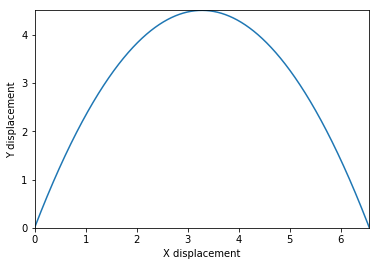
\includegraphics[width=\textwidth,height=\textheight,keepaspectratio]{firstgraph.png}
	\caption{First graph}
\end{figure}
This is perfectly acceptable graph, although it is a bit boring, and the y axis is a bit small, as the top of the graph is cut off slightly. This can be easily fixed by changing line 36 in Listing 3.6 to 
\lstinline[language=Python] $ plt.axis([0, xPos[len(xPos) - 1], 0, max(yPos) + max(yPos) * .2])$. This will increase the height of the axis by the same amount, no matter the launch parameters of the particle, as it is being multiplied by a constant. 

At this point it was decided that questions generated using this graph would be too boring, and simple. So another type of question was chosen similar to this
\begin{figure}[H]
	\centering
	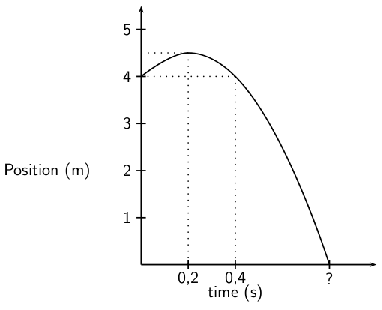
\includegraphics[width=\textwidth,height=\textheight,keepaspectratio]{graph2}
	\caption{Example of a graph \autocite{graph2}}
\end{figure}
This type of graph allows the initial height offset to be randomised, which can make for a more interesting question, and requires some more complex mathematics to solve.

The next generation of the graph was then coded, which meant that particle started at an offset above the ground. Labels were added for the maximum height, and the distance travelled before it hits the ground.
\begin{lstlisting}[language=Python, caption=Second iteration of graph generation]
import matplotlib.pyplot as plt
import numpy as np


def y_displacement(y_offset, initial_speed, theta):
	increment = 0.001
	theta = np.radians(theta)
	x_speed = initial_speed * np.cos(theta)
	y_speed = initial_speed * np.sin(theta)
	x_pos = []
	y_pos = []
	time = 0
	x_pos.append(0)
	
	y_pos.append(y_offset)  # Adding the offset in the first slot of the position array
	
	time += increment
	x_pos_temp = x_speed * time  # Calculating first x value so while loop doesn't fail instantly
	y_pos_temp = (y_speed * time) + (
	0.5 * -9.8 * time ** 2) + y_offset
	
	x_pos.append(x_pos_temp)
	y_pos.append(y_pos_temp)
	
	while y_pos_temp > 0:
		y_pos_temp = (y_speed * time) + (0.5 * -9.8 * time ** 2 + 12)
		x_pos.append(x_speed * time)
		y_pos.append((y_speed * time) + (0.5 * -9.8 * time ** 2) + 12)
		time += increment
		x_distance = max(x_pos)
	plt.plot(x_pos, y_pos)
	plt.annotate(s="", xy=(-1, y_offset), xytext=(-1, 0), arrowprops=dict(arrowstyle='<->'))
	plt.annotate(s="", xy=(0, -1), xytext=(max(x_pos), -1), arrowprops=dict(arrowstyle='<->'))
	plt.plot([0, x_distance], [0, 0], color='k', linestyle='-', linewidth=2)
	plt.plot([0, 0], [0, y_offset], color='k', linestyle='-', linewidth=2)
	plt.plot([-0, -1], [y_offset, y_offset], color='k', linestyle='-', linewidth=2)
	plt.plot([0, x_pos[y_pos.index(max(y_pos))]], [y_offset, y_offset], color='k', linestyle='--', linewidth=2)
	plt.annotate(s="", xy=(x_pos[y_pos.index(max(y_pos))], max(y_pos)),
	xytext=(x_pos[y_pos.index(max(y_pos))], y_offset), arrowprops=dict(arrowstyle='<->'))
	plt.text(-max(x_pos) * 0.08, y_offset / 2, str(y_offset), style='normal')
	plt.text(max(x_pos) / 2, -max(x_pos) * 0.05, str(max(x_pos)), style='normal')
	plt.text(x_pos[y_pos.index(max(y_pos))] + 1, ((max(y_pos) - y_offset) / 2) + y_offset, str(max(y_pos) - y_offset),
	style='normal')
	plt.axis([-5, x_distance, -5, max(y_pos) + 5])
	plt.axis('off')
	plt.show()

y_displacement(12, 20, 30)
\end{lstlisting} 
\begin{figure}[H]
	\centering
	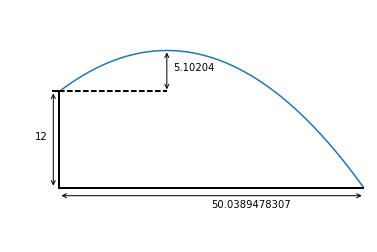
\includegraphics[width=\textwidth,height=\textheight,keepaspectratio]{graph3}
	\caption{Second iteration of graph}
\end{figure}
As you can see this graph is much more interesting that the previous graph. It shows the data needed to answer questions clearly, and it is easy to randomise the variables in it. 

Then questions needed to be designed around this style of graph, so I the questions will be either finding $\theta$, finding the maximum height or finding the distance travelled before it hits the ground. To display these without giving the answer away, I will have to not show some information on the graph depending on the type of question, and also add an indication of which angle $\theta$ is on the graph. 

First I added an arrow showing the initial launch. To draw an arrow you have to give the function two points. The first point was trivial, it was just (0, y offset) however the second point was more involved as it had to be at the right angle. I used trigonometry to work out this point, and the Python code is shown below.
\begin{lstlisting}[language=Python, caption=Arrow coordinate generator]
def calculate_point(start_x, start_y, angle, length):
	endpoint = [start_x + (length * np.cos(angle)), start_y + (length * np.sin(angle))]
	return endpoint
\end{lstlisting}
When you call the function it will return a list of the two coordinates. This can then be used to generate the arrow. This arrow was added with this line of code 
\lstinline[language=Python]|plt.annotate(s="", xy=(0, y_offset), xytext=(calculate_point(0, 12, theta, 10)), arrowprops=dict(arrowstyle='<-'))|
The graph now looks like this:
\insertimage{graph4}{Third iteration of graph}

Next $\theta$ needed to be displayed on the graph. There were three ways to do this, either to draw the symbol manually with a line and an eclipse, use an image of the symbol or use \LaTeX to generate the symbol. I decided to use \LaTeX as it meant that I could easily use other symbols if necessary. 

"LaTeX, which is pronounced «Lah-tech» or «Lay-tech» (to rhyme with «blech» or «Bertolt Brecht»), is a document preparation system for high-quality typesetting. It is most often used for medium-to-large technical or scientific documents but it can be used for almost any form of publishing."\autocite{latex}. This is also what I am using to create this document.

To use \LaTeX with Python is not trivial. You must first get a working installation of \LaTeX on your computer, which is usually done with MikTeX on a Windows machine. Then you must configure matplotlib to use \LaTeX which is done by adding the lines:
\begin{lstlisting}[language=Python, caption=Requirements for \LaTeX in matplotlib]
plt.rc('text', usetex=True) 
plt.rc('font', family='serif') 
\end{lstlisting}
Then to use \LaTeX to display math characters, you must precede the string with \texttt{r}. 
\begin{lstlisting}[language=Python, caption=String used to display $\theta$ using \LaTeX]
r'\textbf{\ensuremath{\theta}'
\end{lstlisting}
The symbol was then added to the graph with this line of code 
\lstinline[language=Python]|plt.text(0 + initial_speed * 0.09, y_offset + initial_speed * 0.02, r'\textbf{\ensuremath{\theta}') |
A label for the initial speed was also added.
\insertimage{graph5}{Fourth iteration of graph}

Finally the angle arc had to be drawn. This was done using Matplotlib patches, which were quite complex. They work essentially like stickers, where you create the item you would like to place, and then you place it at specific coordinates on the graph. The arc was create using this code
\begin{lstlisting}[language=Python, caption=Requirements for \LaTeX in matplotlib]
arc = patches.Arc((0, y_offset), 7, 7,
angle=0, theta1=360, theta2=30, linewidth=1)
\end{lstlisting}
This however is hard coded, so the arc will not change when the angle changes. This can be fixed by changing \lstinline|theta2=30| to \lstinline|theta2=np.degrees(theta)|.
\insertimage{graph6}{Final iteration of graph}
At this point I realised that I would not have enough time to complete the radioactive decay part of the questions, so I decided to focus on the projectile motion questions.

\subsection{Question class}
Once the graph generation was coded, this was put into a class to collect the methods together and make it easy to reuse. The Class created can be found in Algorithm 6 and 7 in Section 2.5
\subsection{GUI Design}
As mentioned before, Qt has a great GUI designer which I will use to create the GUI. Before the GUI was made in QT Creator, the design was prototyped.
\insertimage{hcl}{GUI Design Prototype}
Figure 3.13 is clear and functional. It has large title, so it is clear to the user which topic they are practising. 